\chapter{Shader Local Data: Vertices}

In this chapter we see how to pass per-vertex data to our vertex shader.
To accomplish this task we introduce the concept of vertex buffer.
We also have an in depth look at a technique that allows us to get
the most performance out of a vertex buffer.
At the end, we use the vertex data stored in our vertex buffer to render
a new, fancier, triangle.

\begin{figure}[ht]
    \centering
    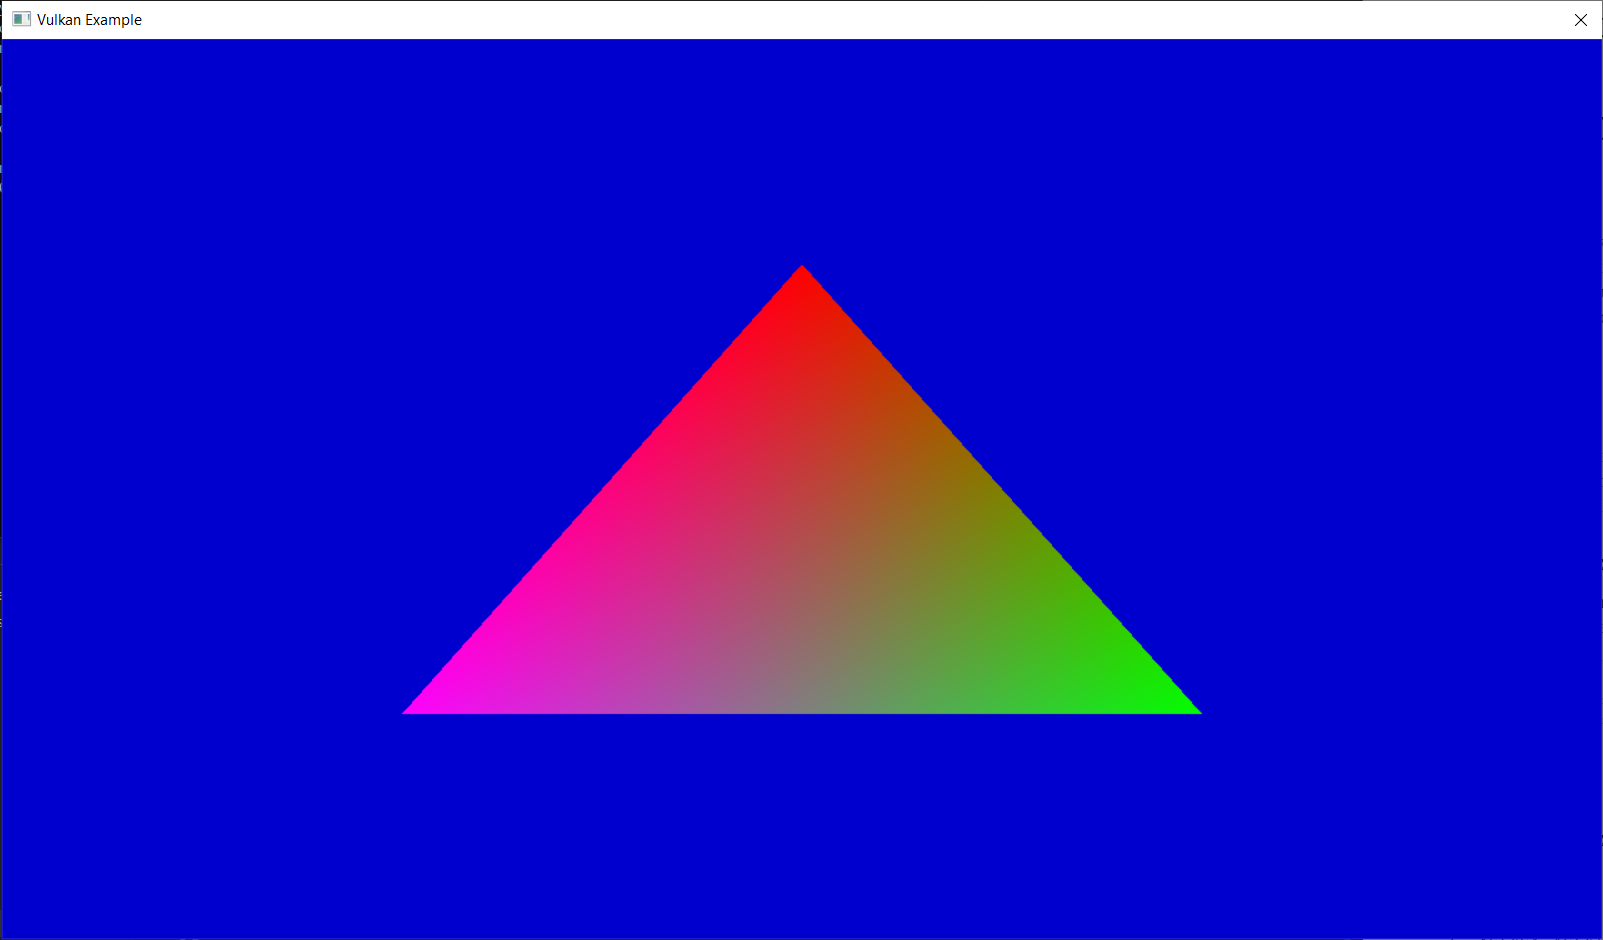
\includegraphics[scale=0.20]{images/ChVertices/RenderTriangle.png}
    \caption{Rendering a triangle}
    \label{fig::RenderTriangleVertices}
\end{figure}

\section{Vertex Data}

In this section we define the vertex data that we will use to draw our triangle.
We will first define the structure of a single vertex.
After that, we will lay out the vertices of our triangle.

\subsection{Vertex}

Here we define the structure of our vertices.
In our case, a vertex stores its 2D position in normalized device coordinates
and its color.

\begin{minipage}{\linewidth}{\noindent}
    \lstinputlisting[
        language=C++,
        caption={What data we store per vertex},
        label={lst::PositionColorVertex}
        ]{src/ChVertices/PositionColorVertex.cpp}
\end{minipage}

\subsection{Vertex Data}

In order to draw a triangle, we specify three vertices.
These are the vertices that will be later uploaded to our GPU and be used
by the graphics pipeline.

\begin{minipage}{\linewidth}{\noindent}
    \lstinputlisting[
        language=C++,
        caption={The vertices that our application will use},
        label={lst::PositionColorVertices}
        ]{src/ChVertices/PositionColorVertices.cpp}
\end{minipage}

\section{Shaders}

We need to write a new vertex and a new fragment shader.
The new vertex shader is due to the fact that we don't use
hardcoded vertex data anymore.
The new vertex shader will also have to handle the fact that
our vertices now store a color value.
The new fragment shader is due to the fact that we use the
vertex color value for our fragment color.

\subsection{Vertex Shader}

Our vertex shader takes as input a position value and a color value.
We also want to pass our vertex color to our fragment shader.

\begin{minipage}{\linewidth}{\noindent}
    \lstinputlisting[
        language=C++,
        caption={Our new vertex shader},
        label={lst::PositionColorShaderVertex}
        ]{src/ChVertices/PositionColorShader.vert}
\end{minipage}

\subsection{Fragment Shader}

Our fragment shader now takes as input the fragment's color.
We use this value to color our fragment.

\begin{minipage}{\linewidth}{\noindent}
    \lstinputlisting[
        language=C++,
        caption={Our new fragment shader},
        label={lst::PositionColorShaderFragment}
        ]{src/ChVertices/PositionColorShader.frag}
\end{minipage}

\section{Upload Vertex Data To The GPU}

Before rendering our triangle, we upload our vertex data to the GPU.
This vertex data will then be passed as input to the graphics pipeline.

\subsection{Understanding The Problem}

Uploading data to the GPU means copying bytes from RAM to GPU memory.
The issue is that we don't know what kind of GPU memory we want to use.

Modern GPUs have different types of memory.
Each GPU memory type has also different memory properties.
There are two memory properties that interest us.
Host visible memory and device local memory.

A host visible memory is a GPU memory that can be mapped to the
application's address space.
A device local memory is a GPU memory that cannot be mapped to the
application's address space.

A host visible memory will always be orders of magnitude slower than a
device local one.
This is due to the fact that a host visible memory must be visible from both
CPU side and GPU side.
This requires particular care from the driver or from the programmer
to keep the data consistent.

Keeping in mind that we don't directly change vertex data at run time,
and that we use said data every frame, we would love to use a memory type
that is device local.
This would improve performance.
The problem is that we still need to upload the vertex data to our GPU,
and to accomplish this task we can only use a memory that is host visible.

\subsection{Our Solution: Idea}

One solution to this problem is to use two buffers.
One buffer, called a staging buffer, will be allocated on host visible
GPU memory.
We use this staging buffer to upload data to the GPU.
The other buffer, called vertex buffer, will be allocated on device local
GPU memory.
After uploading our data to the staging buffer, we issue a memory transfer command
to our GPU.
This command, when executed, will copy the staging buffer's contents
into the vertex buffer.
Later, our vertex buffer will be used by the graphics pipeline for rendering.

\subsection{How To Create A Buffer}

Before implementing our solution we need to know how to cerate a buffer using Vulkan.
Buffer creation is divided in three steps.
We first create a buffer object.
Then, we allocate our buffer memory.
Finally, we bind our buffer memory to our buffer object.

\subsubsection{Create Buffer Object}

The only parameter that can puzzle people is \texttt{sharingMode}.
This is the buffer's sharing mode when it will be accessed by
multiple queue families.
Our buffers are only used by the graphics queue.
Thus, we use the more performant exclusive sharing mode.

\begin{minipage}{\linewidth}{\noindent}
    \lstinputlisting[
        language=C++,
        caption={Create a buffer object},
        label={lst::CreateBuffer}
        ]{src/ChVertices/CreateBuffer.cpp}
\end{minipage}

\subsubsection{Allocate Buffer Memory}

Allocating GPU memory requires some work.
This is due to the fact that modern GPUs have many different types
of memories.
An added complexity is also caused by the fact that we
want our buffer memory to satisfy a given set of memory properties
(host visible, device local, etc ...).

\begin{minipage}{\linewidth}{\noindent}
    \lstinputlisting[
        language=C++,
        caption={Allocate buffer memory},
        label={lst::AllocateBufferMemoy}
        ]{src/ChVertices/AllocateBufferMemoy.cpp}
\end{minipage}

We first need to query our buffer memory requirements.
The query's result contains the set of all memory types that are compatible
with our buffer.

With this information at hand, we pick a memory type on which we will
allocate our buffer memory.
Remember that the memory type we pick must satisfy the memory properties
that we require.
In order to make this process simpler, we use an auxiliary function
called \texttt{FindMemoryType}.
We use \texttt{vkAllocateMemory} to allocate our buffer memory.

\begin{minipage}{\linewidth}{\noindent}
    \lstinputlisting[
        language=C++,
        caption={Find suitable memory type index},
        label={lst::FindMemoryType}
        ]{src/ChVertices/FindMemoryType.cpp}
\end{minipage}

\subsubsection{Bind Buffer Object And Memory}

We use \texttt{vkBindBufferMemory} to bind the buffer's object and
buffer's memory together.

\subsection{Our Solution: Implementation}

Now that we know how to allocate a buffer, we can see how our solution
is implemented.

\subsubsection{Create A Staging Buffer}

We use the \texttt{VK\_BUFFER\_USAGE\_TRANSFER\_SRC\_BIT} flag
because our buffer will be used by the GPU as a source for
transfer operations.

We use the \texttt{VK\_MEMORY\_PROPERTY\_HOST\_VISIBLE\_BIT} flag
because we want our buffer to be host visible.

We use the \texttt{VK\_MEMORY\_PROPERTY\_HOST\_COHERENT\_BIT} flag
because we don't want to manually flush our buffer memory.

\begin{minipage}{\linewidth}{\noindent}
    \lstinputlisting[
        language=C++,
        caption={Crete staging buffer},
        label={lst::CreateStagingBuffer}
        ]{src/ChVertices/CreateStagingBuffer.cpp}
\end{minipage}

\subsubsection{Upload Vertex Data To The Staging Buffer}

Uploading the vertex data to our staging buffer is very simple.
We map the staging buffer memory into our application's address space.
We copy the data.
We unmap the previously mapped memory.

\begin{minipage}{\linewidth}{\noindent}
    \lstinputlisting[
        language=C++,
        caption={Upload our vertex data to the staging buffer},
        label={lst::MapVertexDataIntoStagingBuffer}
        ]{src/ChVertices/MapVertexDataIntoStagingBuffer.cpp}
\end{minipage}

\subsubsection{Create The Vertex Buffer}

We use the \texttt{VK\_BUFFER\_USAGE\_TRANSFER\_DST\_BIT} flag
because our buffer will be used by the GPU as a destination for
transfer operations.

We use the \texttt{VK\_BUFFER\_USAGE\_VERTEX\_BUFFER\_BIT} flag
because our buffer will be used by the GPU as a vertex buffer.

We use the \texttt{VK\_MEMORY\_PROPERTY\_DEVICE\_LOCAL\_BIT} flag
because we want our buffer to be device local.

\begin{minipage}{\linewidth}{\noindent}
    \lstinputlisting[
        language=C++,
        caption={Create vertex buffer},
        label={lst::CreateVertexBuffer}
        ]{src/ChVertices/CreateVertexBuffer.cpp}
\end{minipage}

\subsubsection{Allocate Command Buffer}

We allocate a command buffer from our graphics command pool.
Is it ok to use the graphics command pool to execute transfer commands?
Yes, because all graphics queues always support transfer commands.

\begin{minipage}{\linewidth}{\noindent}
    \lstinputlisting[
        language=C++,
        caption={Allocate our transfer command buffer},
        label={lst::AllocateTransferCommandBuffer}
        ]{src/ChVertices/AllocateTransferCommandBuffer.cpp}
\end{minipage}

\subsubsection{Record Copy Command}

Now we record the memory copy command into our command buffer.
We are telling our GPU to copy \texttt{copyRegion.size} bytes
from our staging buffer to our vertex buffer.

\begin{minipage}{\linewidth}{\noindent}
    \lstinputlisting[
        language=C++,
        caption={Record copy command into our command buffer},
        label={lst::RecordCopyCommand}
        ]{src/ChVertices/RecordCopyCommand.cpp}
\end{minipage}

\subsubsection{Submit Command Buffer}

Now we have to submit our command buffer to the GPU graphics queue.
Doing this will start the execution of our copy command.

\begin{minipage}{\linewidth}{\noindent}
    \lstinputlisting[
        language=C++,
        caption={Submit transfer command buffer},
        label={lst::SubmitCopyCommand}
        ]{src/ChVertices/SubmitCopyCommand.cpp}
\end{minipage}

\subsubsection{Wait For The Command Buffer Execution To Finish}

For simplicity's sake, we wait for our transfer command to finish
before continuing the execution of our application.
To do this we call \texttt{vkQueueWaitIdle} on our graphics queue.
This is not a performance issue, since we should be doing this
only during the application's setup phase.

\subsubsection{Cleanup}

We can now free our command buffer using \texttt{vkFreeCommandBuffers}.
We do this since we won't be using it anymore.
We can also destroy our staging buffer using \texttt{vkFreeMemory}
and \texttt{vkDestroyBuffer}.

\subsection{Review The Process}

Here we can see some pseudocode that outlines all the steps necessary to
create a vertex buffer.

\begin{minipage}{\linewidth}{\noindent}
    \lstinputlisting[
        language=C++,
        caption={Steps for creating our vertex buffer},
        label={lst::VertexBufferCreation}
        ]{src/ChVertices/VertexBufferSolution.cpp}
\end{minipage}

\section{Pipeline Vertex Input State}

During the creation of our pipeline state object, we must specify
the format of the pipeline vertex input data.
To do this we use a \texttt{VkPipelineVertexInputStateCreateInfo} struct.

\texttt{pVertexBindingDescriptions} is an array of vertex input binding descriptions.
\texttt{pVertexAttributeDescriptions} is an array of vertex input attribute descriptions.

\begin{minipage}{\linewidth}{\noindent}
    \lstinputlisting[
        language=C++,
        caption={Describe the pipeline input data},
        label={lst::VkPipelineVertexInputStateCreateInfo}
        ]{src/ChVertices/VkPipelineVertexInputStateCreateInfo.cpp}
\end{minipage}

\subsection{Binding Descriptions}

A \texttt{VkVertexInputBindingDescription} struct has three fields.
\texttt{binding} is the binding number that this structure describes.
\texttt{stride} is the number of bytes between consecutive elements within the
vertex buffer.
\texttt{inputRate} is a value that specifies whether vertex attribute addressing
is a function of the vertex index or of the instance index.

Some of you may be wondering: what is a vertex input binding?
Before recording a draw command into a command buffer,
we must bind a vertex buffer in order for our pipeline to use it.
We use \texttt{vkCmdBindVertexBuffers} to do this.
This function takes an array of buffers.
This is because our pipeline can get vertex data from multiple buffers
at the same time.
\texttt{binding} is an index into the \texttt{pBuffers} array bound by
\texttt{vkCmdBindVertexBuffers}.

In our case, all the vertex data is packed together and comes from a single buffer.
Hence, we only have one binding description.

\begin{minipage}{\linewidth}{\noindent}
    \lstinputlisting[
        language=C++,
        caption={Describe our vertex input bindings},
        label={lst::VkVertexInputBindingDescription}
        ]{src/ChVertices/VkVertexInputBindingDescription.cpp}
\end{minipage}

\subsection{Attribute Descriptions}

A vertex attribute is an input variable that is supplied per-vertex to a shader.
In our case, for each vertex, we pass into our shader a position and a color.
Thus, in our case, a vertex has two attributes: a position attribute and a
color attribute.

Before creating our pipeline state object we must describe all our
vertex attributes.
We do this using an array of \texttt{VkVertexInputAttributeDescription} struct
instances.
\texttt{location} is the shader input location number for this attribute.
We have seen this value earlier when we wrote \texttt{layout(location = 0)}
in our vertex shader.
\texttt{binding} is the binding number which this attribute takes its data from.
\texttt{format} is the size and type of the vertex attribute data.
\texttt{offset} is the byte offset of this attribute relative to the start of
an element in the vertex input binding.

\begin{minipage}{\linewidth}{\noindent}
    \lstinputlisting[
        language=C++,
        caption={Describe our vertex input attributes},
        label={lst::VkVertexInputAttributeDescription}
        ]{src/ChVertices/VkVertexInputAttributeDescription.cpp}
\end{minipage}

\section{Draw Using Our Vertex Data}

The only missing thing now is to tell Vulkan to render a triangle using our
vertex data.
We do this during our rendering command buffer recording.

\begin{minipage}{\linewidth}{\noindent}
    \lstinputlisting[
        language=C++,
        caption={Draw triangle using our vertex data},
        label={lst::DrawWithVertexBuffer}
        ]{src/ChVertices/DrawWithVertexBuffer.cpp}
\end{minipage}
